\section{Results}
We first turn our attention to the results of the cluster-abstraction algorithm. 
In table \ref{aha-table:graphsize} we present the average size of the abstract graph in nodes and edges and contrast it to the size of the original graph which featured an average of 4469 nodes and 16420 edges. In addition to comparing performance 
compared to the size of the original graph. 
\begin{figure}[htbp]
       \caption{\emph{AHA* performance (high vs low quality abstraction). Top: Path quality. Bottom: Search effort. }}
       \begin{center}
                       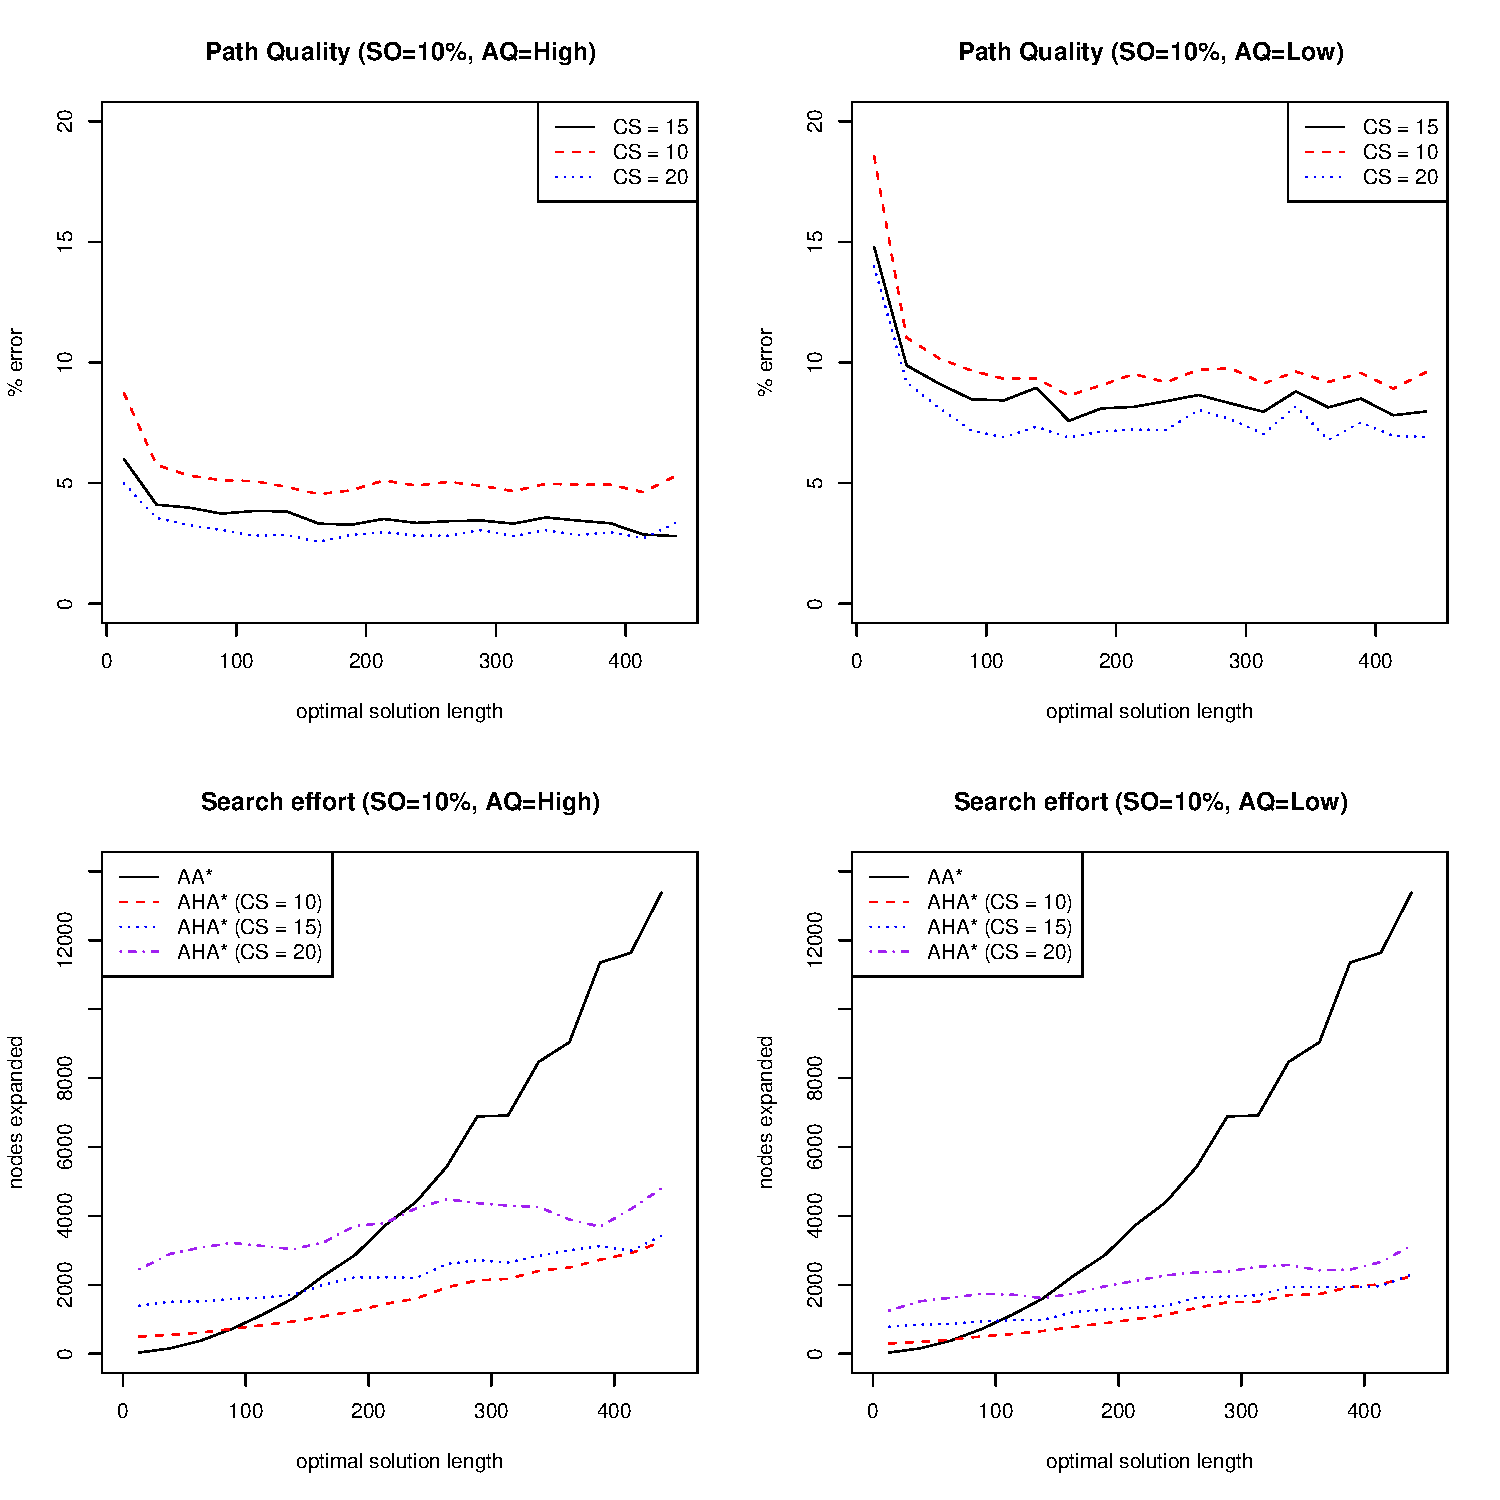
\includegraphics[scale=0.35]{diagrams/allgraphs.pdf}
       \end{center}
       \label{aha-fig:allgraphs}
\end{figure}
\input gsntable.tex
stuff stuf stuff
stuff stuf stuff
stuff stuf stuff
stuff stuf stuff
stuff stuf stuff
stuff stuf stuff
stuff stuf stuff
stuff stuf stuff
stuff stuf stuff
stuff stuf stuff
stuff stuf stuff
stuff stuf stuff
stuff stuf stuff
stuff stuf stuff
stuff stuf stuff
stuff stuf stuff
stuff stuf stuff
stuff stuf stuff
stuff stuf stuff
\input pqtable.tex
stuff stuf stuff
stuff stuf stuff
stuff stuf stuff
stuff stuf stuff
stuff stuf stuff
stuff stuf stuff
stuff stuf stuff
stuff stuf stuff
\input setable.tex
stuff stuf stuff
stuff stuf stuff
stuff stuf stuff
stuff stuf stuff
stuff stuf stuff
stuff stuf stuff
stuff stuf stuff
